\documentclass{beamer}


\usepackage[spanish]{babel}
\usepackage[T1]{fontenc}
\usepackage[utf8]{inputenc}

\usepackage{graphics}
\graphicspath{{img/}}

\usetheme{Madrid}
\usecolortheme{beaver}
\setbeamercovered{transparent}

% \usepackage{beamerthemesplit} // Activate for custom appearance

\title{Modelación Basada en Agentes}
\author{Dr. Felipe Contreras}
\date{\today}

\begin{document}

\frame{\titlepage}

\section[Outline]{}
\frame{\tableofcontents}

\section{Antecedentes}

\subsection{Sistemas Complejos}
\frame{\alert{Sistemas Complejos}}
  \setbeamercovered{transparent}
\begin{frame}[t]
  \frametitle{Características}
  \begin{itemize}[<+-| alert@+>]
  \item Sistema: Conjunto de elementos o partes conectadas entre sí, que llevan acabo cierta función
  \item Complejo $\neq$ Complicado
  \item Presentan auto-organización
  \item Exhiben propiedades emergentes (``el todo es más que la suma de sus partes'')
  \begin{enumerate}[<+-| alert@+>]
  \item Muchos elementos
  \item Las interacciones son dinámicas
  \item Elementos influyen y son influidos por los demás
  \item Las interacciones son no lineales (pequeñas ``causas'', pueden tener ``efectos'' grandes)
  \item Las interacciones son recursivas
  \item Son abiertos % interacturan con otros sistemas
  \item Operan lejos del equilibrio
  \item Tienen una historia
  \item Los elementos actúan con información local
  \end{enumerate}
  \end{itemize}
  \end{frame}

\subsection{Mapeos Discretos}
\frame{\alert{Mapeos Discretos}}
\frame{
  \frametitle{Mapeos discretos}
  \begin{itemize}[<+->]
  \item $y = f(x)$
  \item $x_{1} = f(x_{0})$
  \item $x_{2} = f(x_{1}), x_{3}=f(x_{2}), x_{4} = f(x_{3}), ...$
  \end{itemize}
}
\frame{\frametitle{Representación gráfica}
\begin{block}{}
\begin{center}
\includegraphics<+>[height=.5\textheight]{mapeo1}
\includegraphics<+>[height=.5\textheight]{mapeo2}
\only<3>{ Programa ``logistica''}
\includegraphics<+>[width=.8\textwidth]{mapeo3}
\end{center}
\end{block}
}
\frame
{
  \frametitle{Características}

  \begin{itemize}[<+->]
  \item Converge (a un punto)
  \item No converge: tiene ciclo límite
  \item No converge: órbita densa
  \end{itemize}
}

\subsection{Autómatas Celulares}
\frame{\alert{Autómatas Celulares}}

\begin{frame}[t]
  \frametitle{Definición (genérica)}
  \begin{itemize}[<+->]
  \item Un AC consiste de autómatas (llamados también celdas o sitios) idénticos, dispuestos uniformemente en los puntos de una látice $D$-dimensional de un espacio discreto. Normalmente D=$1, 2,$ o $3$
  \item Cada autómata es una variable dinámica y su cambio temporal esta dado por la expresión:
  $$s_{t+1}(x) = F (s_{t}(x + x_{0}), s_{t}(x + x_{1}),\ldots , s_{t}(x + x_{n-1}))$$
  \item $s_{t}(x)$ es el estado de un autómata localizado en $x$ en el tiempo $t$
  \item $F$ es la función de transición de estado
  \item y $N=\{x_{0}, x_{1}, \ldots, x_{n-1}\}$ es la \textit{vecindad}
  \item por lo general se aplica la misma $F$ y la misma vecindad uniformemente a todas las posiciones espaciales
  \end{itemize}
\end{frame}

\begin{frame}[t]
  \frametitle{Definición (genérica)}
  \begin{itemize}[<+->]
  \item Fueron inicialmente desarrolladas por John von Newmann y su colaborador Stanislaw Ulam 
  \item Constituyen una forma de describir dinámicas espacio-temporales altamente no lineales de una manera simple y concisa
  \item Se utilizan para diversos campos como la dinámica molecular, hidrodinámica, propiedades físicas de materiales, procesos químicos de reacción-difusión, crecimiento y morfogénesis de organismos vivos, etc. [Sayama p.185 y ss]
  \end{itemize}
\end{frame}

\begin{frame}[t]
  \frametitle{AC 1D: Definición práctica}
  \begin{columns}[t]
  \column{.5\textwidth}
  \begin{block}{}
	\begin{itemize}[<+->]
		\item Vocabulario $\sigma$ de $n$ símbolos
		\item Organización de $m$ de estos símbolos en un estado inicial $E_{0}$
		\item Tamaño de vecindad o radio $\rho$
		\item Condiciones en la frontera (cíclica, terminación, valor único)
		\item Regla de evolución (función de mapeo)
	\end{itemize}
  \end{block}
   \column{.5\textwidth}
  \begin{center}
	\only<1> {$\sigma = \{0, 1\}$, $n=2$}
	\includegraphics<2>[width=.9\textwidth]{automata1}
	\only<3> {$\rho=3$}
	\includegraphics<4>[width=.9\textwidth]{automata2}
	\includegraphics<5>[height=.4\textheight]{automata3}
  \end{center}
  \end{columns}
\end{frame}

\begin{frame}[t]
  \frametitle{Regla de evolución}
  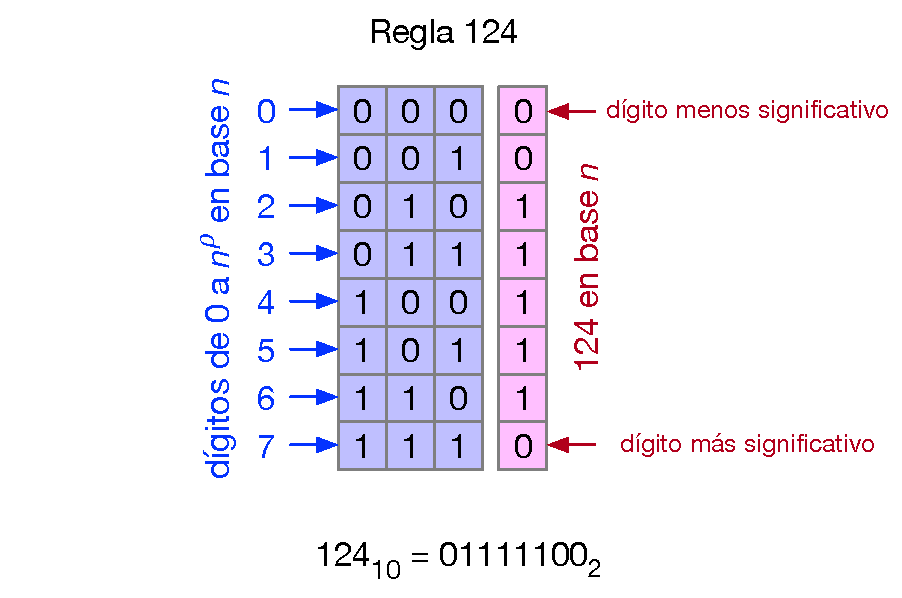
\includegraphics[width=.9\textwidth]{automata4}
\end{frame}

\begin{frame}[t]
  \frametitle{Aplicación de la regla}
  \includegraphics<+>[width=.9\textwidth]{automata51}
  \includegraphics<+>[width=.9\textwidth]{automata52}
  \includegraphics<+>[width=.9\textwidth]{automata53}
  \includegraphics<+>[width=.9\textwidth]{automata54}
  \includegraphics<+>[width=.9\textwidth]{automata55}
  \includegraphics<+>[width=.9\textwidth]{automata56}
  \includegraphics<+>[width=.9\textwidth]{automata57}
  \includegraphics<+>[width=.9\textwidth]{automata58}
  \includegraphics<+>[width=.9\textwidth]{automata59}
  \only<+>{?`cómo quedan las demás?, ?`cómo funciona la condición de frontera cíclica?}
\end{frame}

\begin{frame}[t]
  \frametitle{Ejemplos (Programa ``Autómatas Celulares'')}
  \begin{center}
  \only<+> {Regla 90, $E_{0}$=``central'' }
  \only<+> {Regla 94, $E_{0}$=``01110000000000001111100001111'' }
  \only<+> {Regla 135, $E_{0}$=``azar'' }
  \end{center}
  \begin{center}
  \includegraphics<1>[height=.6\textheight]{ac11}
  \includegraphics<2>[height=.6\textheight]{ac12}
  \includegraphics<3>[height=.6\textheight]{ac13}
  \end{center}
\end{frame}

\begin{frame}[t]
\frametitle{Clasificación de Wolfram}
\begin{itemize}[<+-| alert@+>]
	\item Uniforme
	\item Cíclico
	\item Aleatorio
	\item Complejo
\end{itemize}
\end{frame}

\begin{frame}[t]
  \frametitle{Autómatas en 2D: El juego de la vida}
  \begin{itemize}[<+->]
  \item {El conjunto de símbolos es $\sigma=\{0,1\}$, significando 0=``muerta'', 1=``viva''}
  \item {$E_{0}$, y todos los demás estados, están dispuestos en una parrilla 2D de celdas}
  \item {La vecindad mide $\rho=(3,3)$, es un cuadro de $3\times 3$ símbolos}
  \item {La regla de evolución para el siguiente estado, asigna a la celda central el valor:}
  \begin{itemize}[<+->]
  \item ``viva'', si la celda central esta ``muerta'' y hay exactamente 3 vecinos vivos
  \item ``muerta'', si la celda central está ``viva'' y más de 3 (sobrepoblación) o menos de 2 (soledad) vecinos están vivos
  \item En cualquier otro caso, la celda mantiene su símbolo
  \end{itemize}
  \end{itemize}
  \begin{center}\includegraphics<+>[width=.6\textwidth]{vida1}\end{center}
\end{frame}

\begin{frame}[t]
\frametitle{Autómatas en 2D: Regla de la mayoría}
\begin{itemize}[<+->]
	\item La vida o muerte de la celda central está dictada por el valor de la mayoría de las celdas de su vecindad de Moore
\end{itemize}
\begin{center}
	\includegraphics<1>[width=.3\textwidth]{moore}
	\only<2> {Programa ``Manchas''}
	
	\includegraphics<2>[width=.5\textwidth]{manchas}
\end{center}
\end{frame}

\begin{frame}[t]
\frametitle{Autómatas en 2D: Patrones de Turing}
\begin{columns}[t]
	\column{.7\textwidth}
	\begin{itemize}[<+->]
	\item Dos regiones elípticas, concéntricas a la celda central, cuya vida determinan
	\item Las celdas vivas en la elipse interna constituyen los activadores ($A$)
	\item Las celdas fuera de la elipse interna pero dentro de la externa constituyen los inhibidores ($I$)
	\item Hay un factor $w$ que dice que tan potentes son los inhibidores respecto a los activadores ($w=2$, significa que son el doble de potentes)
	\item Calcular $F = A - w * I$
	\begin{itemize}[<+->]
		\item Si $F >0$, la celda central vive
		\item Si $F<0$, la celda central muere
		\item Si $F=0$,  la celda central no cambia su valor
	\end{itemize}
	\end{itemize}
	\column{.3\textwidth}
	\begin{center}
		\includegraphics<1->[width=.9\textwidth]{fur1}
	\end{center}
\end{columns}
\end{frame}

\begin{frame}[t]
\frametitle{Autómatas en 2D: Patrones de Turing}
\begin{center}
	Programa ``Fur'' (biblioteca de modelos de Netlogo)
	
	\includegraphics<+>[width=.6\textwidth]{fur2}
\end{center}
\end{frame}



\end{document}